% Template of basic phisics experiment 基于 article template, 在此基础上做修改
% 设定文章编码类型, 正文字号为五号则 zihao=5, 正文字号为小四则 zihao=-4
\documentclass[zihao=5, UTF8]{article}		


% 自定义宏定义
\def\N{\mathbb{N}}
\def\F{\mathbb{F}}
\def\Z{\mathbb{Z}}
\def\Q{\mathbb{Q}}
\def\R{\mathbb{R}}
\def\C{\mathbb{C}}
\def\T{\mathbb{T}}
\def\S{\mathbb{S}}
\def\A{\mathbb{A}}
\def\I{\mathscr{I}}
\def\d{\mathrm{d}}
\def\p{\partial}


% 物理实验报告所需的其它宏包
\usepackage{ulem}   % \uline 下划线支持

% 导入基本宏包
\usepackage[UTF8]{ctex}     % 设置文档为中文语言
\usepackage[colorlinks, linkcolor=blue, anchorcolor=blue, citecolor=blue, urlcolor=blue]{hyperref}  % 宏包：自动生成超链接 (此宏包与标题中的数学环境冲突)
% \usepackage{docmute}    % 宏包：子文件导入时自动去除导言区, 用于主/子文件的写作方式, \include{./51单片机笔记}即可. 注：启用此宏包会导致.tex文件capacity受限. 
\usepackage{amsmath}    % 宏包：数学公式
\usepackage{mathrsfs}   % 宏包：提供更多数学符号
\usepackage{amssymb}    % 宏包：提供更多数学符号
\usepackage{pifont}     % 宏包：提供了特殊符号和字体
\usepackage{extarrows}  % 宏包：更多箭头符号

% 列表环境设置
\usepackage{enumitem}   % 宏包：列表环境设置
    \setlist[enumerate]{itemsep=0pt, parsep=0pt, topsep=0pt, partopsep=0pt, leftmargin=3.5em} 
    \setlist[itemize]{itemsep=0pt, parsep=0pt, topsep=0pt, partopsep=0pt, leftmargin=3.5em}
    \newlist{circledenum}{enumerate}{1} % 创建一个新的枚举环境  
    \setlist[circledenum,1]{  
        label=\protect\circled{\arabic*}, % 使用 \arabic* 来获取当前枚举计数器的值, 并用 \circled 包装它  
        ref=\arabic*, % 如果需要引用列表项, 这将决定引用格式（这里仍然使用数字）
        itemsep=0pt, parsep=0pt, topsep=0pt, partopsep=0pt, leftmargin=3.5em
    }  
% 文章页面 margin 设置
\usepackage[a4paper]{geometry}  % 宏包：文章页面 margin 设置
    \geometry{top=0.75in}
    \geometry{bottom=0.75in}
    \geometry{left=0.75in}
    \geometry{right=0.75in}   % 设置上下左右页边距
    \geometry{marginparwidth=1.75cm}    % 设置边注距离（注释、标记等）

% 自定义数学环境
\usepackage{amsthm} % 宏包：数学环境配置
% theorem-line 环境自定义
    \newtheoremstyle{MyLineTheoremStyle}% <name>
        {11pt}% <space above>
        {11pt}% <space below>
        {}% <body font> 使用默认正文字体
        {}% <indent amount>
        {\bfseries}% <theorem head font> 设置标题项为加粗
        {：}% <punctuation after theorem head>
        {.5em}% <space after theorem head>
        {\textbf{#1}\thmnumber{#2}\ \ (\,\textbf{#3}\,)}% 设置标题内容顺序
    \theoremstyle{MyLineTheoremStyle} % 应用自定义的定理样式
    \newtheorem{LineTheorem}{Theorem.\,}
% theorem-block 环境自定义
    \newtheoremstyle{MyBlockTheoremStyle}% <name>
        {11pt}% <space above>
        {11pt}% <space below>
        {}% <body font> 使用默认正文字体
        {}% <indent amount>
        {\bfseries}% <theorem head font> 设置标题项为加粗
        {：\\ \indent}% <punctuation after theorem head>
        {.5em}% <space after theorem head>
        {\textbf{#1}\thmnumber{#2}\ \ (\,\textbf{#3}\,)}% 设置标题内容顺序
    \theoremstyle{MyBlockTheoremStyle} % 应用自定义的定理样式
    \newtheorem{BlockTheorem}[LineTheorem]{Theorem.\,} % 使用 LineTheorem 的计数器
% definition 环境自定义
    \newtheoremstyle{MySubsubsectionStyle}% <name>
        {11pt}% <space above>
        {11pt}% <space below>
        {}% <body font> 使用默认正文字体
        {}% <indent amount>
        {\bfseries}% <theorem head font> 设置标题项为加粗
        {：\\ \indent}% <punctuation after theorem head>
        {0pt}% <space after theorem head>
        {\textbf{#3}}% 设置标题内容顺序
    \theoremstyle{MySubsubsectionStyle} % 应用自定义的定理样式
    \newtheorem{definition}{}


% 有色文本框及其设置
\usepackage[dvipsnames,svgnames]{xcolor}    %设置插入的文本框颜色
\usepackage[strict]{changepage}     % 提供一个 adjustwidth 环境
\usepackage{framed}     % 实现方框效果
    \definecolor{graybox_color}{rgb}{0.95,0.95,0.96} % 文本框颜色. 修改此行中的 rgb 数值即可改变方框纹颜色, 具体颜色的rgb数值可以在网站https://colordrop.io/ 中获得. （截止目前的尝试还没有成功过, 感觉单位不一样）（找到喜欢的颜色, 点击下方的小眼睛, 找到rgb值, 复制修改即可）
    \newenvironment{graybox}{%
    \def\FrameCommand{%
    \hspace{1pt}%
    {\color{gray}\small \vrule width 2pt}%
    {\color{graybox_color}\vrule width 4pt}%
    \colorbox{graybox_color}%
    }%
    \MakeFramed{\advance\hsize-\width\FrameRestore}%
    \noindent\hspace{-4.55pt}% disable indenting first paragraph
    \begin{adjustwidth}{}{7pt}%
    \vspace{2pt}\vspace{2pt}%
    }
    {%
    \vspace{2pt}\end{adjustwidth}\endMakeFramed%
    }

% 各级标题自定义设置
\usepackage{titlesec}   
    % section标题自定义设置 
    \titleformat{\section}[hang]{\normalfont\huge\bfseries\centering}{第\,\thesection\,部分}{20pt}{}
    % subsection标题自定义设置 
    \titleformat{\subsection}[hang]{\normalfont\Large\bfseries}{\,\thesubsection\,}{8pt}{}
    % subsubsection标题自定义设置
    \titleformat{\subsubsection}[hang]{\normalfont\large\bfseries}{\,\thesubsubsection\,}{6pt}{}

% 外源代码插入设置
\usepackage{matlab-prettifier}
    \lstset{
        style=Matlab-editor,  % 继承matlab代码颜色等
    }
\usepackage[most]{tcolorbox} % 引入tcolorbox包 
\usepackage{listings} % 引入listings包
    \tcbuselibrary{listings, skins, breakable}
    \lstdefinestyle{matlabstyle}{
        language=Matlab,
        basicstyle=\small,
        breakatwhitespace=false,
        breaklines=true,
        captionpos=b,
        keepspaces=true,
        numbers=left,
        numbersep=15pt,
        showspaces=false,
        showstringspaces=false,
        showtabs=false,
        tabsize=2
    }
    \newtcblisting{matlablisting}{
        arc=0pt,
        top=0pt,
        bottom=0pt,
        left=1mm,
        listing only,
        listing style=matlabstyle,
        breakable,
        colback=white   % 选一个合适的颜色
    }

% table 支持
\usepackage{booktabs}   % 宏包：三线表
\usepackage{tabularray} % 宏包：表格排版
\usepackage{longtable}  % 宏包：长表格

% figure 设置
\usepackage{graphicx}  % 支持 jpg, png, eps, pdf 图片 
\usepackage{svg}       % 支持 svg 图片
    \svgsetup{
        % 指向 inkscape.exe 的路径
        inkscapeexe = C:/aa_MySame/inkscape/bin/inkscape.exe, 
        % 一定程度上修复导入后图片文字溢出几何图形的问题
        inkscapelatex = false                 
    }


% 图表进阶设置
\usepackage{float}     % 图表位置浮动设置 
\usepackage{caption}    % 图注、表注
    \captionsetup[figure]{name=图}  
    \captionsetup[table]{name=表}
    \captionsetup{labelfont=bf, font=small}

% 文章默认字体设置
    \usepackage{fontspec}   % 宏包：字体设置
        \setmainfont{SimSun}[
            BoldFont = SimHei, % 设置粗体字为黑体
            ItalicFont = KaiTi, % 设置斜体字为楷体
            BoldItalicFont = KaiTi % 设置粗斜体字为楷体
        ] 
        %\setCJKmainfont[AutoFakeBold=3]{SimSun} % 设置加粗字体为 SimSun 族, AutoFakeBold 可以调整字体粗细
        \setmainfont{Times New Roman} % 设置英文字体为Times New Roman


% 其它设置
    % equation 公式编号设置
        \makeatletter  
        \renewcommand{\theequation}{\thesection.\arabic{equation}}  
        \makeatother
    % 脚注设置
        \renewcommand\thefootnote{\ding{\numexpr171+\value{footnote}}}
    % 参考文献引用设置
        \bibliographystyle{unsrt}   % 设置参考文献引用格式为unsrt
        \newcommand{\upcite}[1]{\textsuperscript{\cite{#1}}}     % 自定义上角标式引用
    % 文章序言设置
        \newcommand{\cnabstractname}{序言}
        \newenvironment{cnabstract}{%
            \par\Large
            \noindent\mbox{}\hfill{\bfseries \cnabstractname}\hfill\mbox{}\par
            \vskip 2.5ex
            }{\par\vskip 2.5ex}


% 页眉页脚设置
\usepackage{fancyhdr}   %宏包：页眉页脚设置
    \pagestyle{fancy}
    \fancyhf{}
    \cfoot{\thepage}
    \renewcommand\headrulewidth{1pt}
    \renewcommand\footrulewidth{0pt}
    \rhead{\bfseries 分组序号: 3-04-1}    
    \chead{《基础物理实验》实验报告,\ 潘天麟\ 2023K8009908023}
    \lhead{2024.10.16}

% 开始编辑文章

\begin{document}
\noindent\begin{flushright}
    \zihao{2}{分组序号: 3-04-1}
\end{flushright}

\setCJKfamilyfont{boldsong}[AutoFakeBold = {2.17}]{SimSun}
\newcommand*{\boldsong}{\CJKfamily{boldsong}}


\begin{center}\large
    \noindent{\Huge\bfseries\boldsong《基础物理实验》实验报告 }
    \\\vspace{0.4cm}
    \noindent\textit{
        \textbf{\boldsong 实验名称：}\uline{\hspace{2.3cm} 微波干涉衍射实验\hspace{2.3cm}}\hspace{0.4cm} 
        指导教师：\uline{\hspace{1.5cm}刘荣鹃\hspace{1.5cm}}}
    \\\vspace{0.1cm}
    \noindent\textit{
        姓名：\uline{\,\,潘天麟\,\,}\hspace{0.2cm}
        学号：\uline{\,\,{\upshape 2023K8009908023}\,\,}\hspace{0.2cm}
        专业：\uline{\,\,人工智能\,\,}\hspace{0.2cm}
        班级：\uline{\,\,\upshape{2313}\,\,}\,组号：\uline{\,\,\upshape{3-04-1}\,\,}}
    \\\vspace{0.1cm}
    \noindent\textit{
        实验日期：\uline{\,\,{\upshape 2024.10.16}\,\,}\hspace{0.2cm}
        实验地点：\uline{\,\,\,教学楼{\upshape717}\,\,\,}\hspace{0.2cm}
        是否调课/补课：\uline{\hspace{1.3cm}}\hspace{0.2cm}
        成绩：\uline{\hspace{2cm}}}
\end{center}
% \vspace{-0.2cm}
\noindent\rule{\textwidth}{0.1em}   % 分割线

\section{实验目的}
\begin{enumerate}
    \item 了解与学习微波产生的基本原理以及传播和接收等基本特性. 
    \item 观测微波衍射、干涉等实验现象. 
    \item 观测模拟晶体的微波布拉格衍射现象. 
    \item 通过迈克耳逊实验测量微波波长. 
\end{enumerate}
\section{实验仪器}
DHMS-1型微波光学综合实验仪, 包括：X波段微波信号源、微波发生器、射喇叭、接收喇叭、微波检波器、检波信号数字显示器、可旋转载物平台和支架, 以及实验用附件（反射板、分束板、单缝板、双缝板、晶体模型、读数机构等）. 
\section{实验原理}
\subsection{微波的产生和接收}
本实验所采用的微波发生器通过电调制技术实现功能. 其内部装有一个电压可调的压控振荡器（VCO）, 能够产生4.4 GHz至5.2 GHz的信号. 该信号的输出频率会根据输入电压的不同而变化. 信号经过滤波器后, 提取出8.8 GHz至9.8 GHz的二次谐波, 经过适当衰减和放大处理, 再通过隔离器, 由探针输出至波导口, 最终由E面天线发射. 

接收系统则采用了检波与数显一体化设计. E面喇叭天线负责接收微波信号, 并将其传递给高灵敏度的检波管, 将微波信号转换为电信号. 随后, 通过穿心电容输出检波电压, 经过A/D转换, 最终在液晶显示器上显示微波的相对强度. 

\subsection{微波布拉格衍射实验}
\subsubsection{晶体结构}    

组成晶体的原子或分子按照一定的规律在空间中进行周期性的排列是晶体的基本结构. 这种排列最基础的形式是原子在直角坐标系中沿着$x$、$y$、$z$三个坐标轴, 以固定的距离$a$进行有序的空间重复, 从而形成了一个简单的立方点阵结构. 这个固定的原子间距$a$被我们称为\textit{晶格常数}. 在晶体中, 原子可以被视作位于一系列相互平行且间距恒定的平面族上, 这些平面我们称之为\textit{晶面}. 

晶面的选取有多种方式, 而在众多晶面中, 最为关键且频繁使用的有三种, 即（100）面、（110）面和（111）面. 这些晶面通过圆括号中的三个数字来标识, 这些数字称为晶面指数. 具体来说, （100）面的法线方向与坐标轴一致, 相邻两个（100）面之间的距离正好等于晶格常数$a$. 对于（110）面, 其法线方向沿着坐标平面中正方形的对角线, 因此相邻两个（110）面的间距为$\frac{a}{\sqrt{2}}$. 而（111）面的法线方向则沿着正立方体的体对角线, 相邻两个（111）面的间距为$\frac{a}{\sqrt{3}}$. 

除了这些基本的晶面, 还存在许多其他更复杂的晶面取法, 它们形成了不同取向的晶面族. 通常情况下, 对于晶面指数为$(n_1, n_2, n_3)$的晶面族, 其相邻两个晶面的间距可以用公式$d=\frac{a}{\sqrt{n_1^2+n_2^2+n_3^2}}$来计算. 

\subsubsection{布拉格衍射}
晶体在三维空间中原子的格点可以看做是一个三维的光栅网络, 晶体对电子波衍射的可以由每个格点上的原子产生的散射波的相干叠加得到, 相干叠加的过程可以分为两步
\begin{enumerate}
    \item 一个晶面上各个原子发出散射波的相干叠加  
    \item 同一晶面族的不同晶面的衍射波之间的相干叠加
\end{enumerate}

处在同一平面上的原子组成一个晶面, 它们的散射波相干叠加的结果遵从反射定律, 即反射角等于入射角；而从间隔为 $d$ 的相邻两个晶面反射的两束波的程差就是 $2d\sin\theta$, 其中$\theta$ 为入射角与晶面的夹角. 则当
\begin{equation}
2d \sin\theta = k\lambda, \quad k=1, 2, 3, \cdots 
\end{equation}
时, 达到干涉极大, 方程（1）称为晶体衍射的\textit{布拉格条件}. 如果改成通常习惯的入射角 $\beta$ 表示, 布拉格条件可写为：

\begin{equation}
2d \cos\beta = k\lambda, \quad k=1, 2, 3, \cdots 
\end{equation}

根据这个公式, 如果我们在每一晶面从实验上测得衍射极大的方向角 $\beta$, 已知晶格常数 $a$, 则可以求出晶面间距 $d$, 进而可求出波长 $\lambda$. 

\subsection{微波的单缝衍射实验(未做)}
当平面微波入射到一个宽度与微波波长相近的一个狭缝时, 在缝后会发生衍射现象. 中央零级最强最宽, 在中央的两侧衍射波强度将迅速减小. 微波单缝衍射图样的强度分布函数为
\begin{equation}
I = I_0 \frac{\sin^2 \mu}{\mu^2}, \quad \mu = \frac{\pi \alpha \sin \phi}{\lambda}
\end{equation}
其中 $I_0$ 是中央主极大中心的微波强度, $\alpha$ 为单缝的宽度, $\lambda$ 为微波的波长, $\phi$ 为衍射角, $\frac{\sin^2 \mu}{\mu^2}$ 常叫做单缝衍射因子表征衍射场内任一点微波相对强度的大小. 当
\begin{equation}
\alpha \sin \phi = \pm k \lambda, \quad k = 1, 2, 3, 4, \ldots
\end{equation}
时, 相应的 $\phi$ 角位置衍射度强度为零. 如测出衍射强度分布, 则可依据第一级衍射最小值所对应的 $\phi$ 角度, 利用公式（4）, 求出微波波长 $\lambda$. 

\subsection{微波的双缝干涉实验}
当一平面波垂直入射到一金属板的两条狭缝上, 狭缝就成为次级波波源. 由两缝发出的次级波是相干波, 因此在金属板的背后面空间中, 将产生干涉现象. 为了只研究主要来自两缝中央衍射波相互干涉的结果, 令双缝的缝宽 $a$ 接近 $\lambda$, 由于每个缝在波通过时都有衍射现象, 要让两缝之间的间隔 $b$ 较大, 这样干涉强度受单缝衍射的影响小, 其中干涉加强的角度为：
\begin{equation}
\phi = \arcsin \left( \frac{k \lambda}{a+b} \right), \quad k = 1, 2, 3, \ldots
\end{equation}
干涉减弱的角度为：
\begin{equation}
\phi = \arcsin \left[ \frac{(2k + 1) \lambda}{2(a + b)} \right], \quad k = 1, 2, 3, \ldots
\end{equation}
根据干涉加强和减弱的角度, 就可以推算出波长 $\lambda$ 的大小. 

\subsection{微波的迈克尔逊干涉实验}
在微波前进的方向上放置一个与波传播方向成 $45^\circ$ 角的半透射半反射的分束板. 将入射波分成一束向金属板 A 传播, 另一束向金属板 B 传播. 由于 A、B 金属板的全反射作用, 两列波再回到半透射半反射的分束板, 回合后到达微波接收器处. 这两束微波同频率, 在接收器处将发生干涉, 干涉叠加的强度由两束波的程差（即位相差）决定. 当两波的相位差为 $2k\pi$ ($k = \pm 1, \pm 2, \pm 3, \ldots$) 时, 干涉加强；

当两波的相位差为 $(2k + 1)\pi$ 时, 干涉最弱. 当 A、B 板中的一块板固定, 另一块板可沿着微波传播方向前后移动, 当微波接收信号从极小（或极大）值到又一次极小（或极大）值, 则反射板移动了 $\frac{\lambda}{2}$ 距离. 由这个距离就可求得微波波长 $\lambda$. 

\subsection{微波的偏振实验(未做)}
电磁波是横波, 它的电场强度矢量 $\boldsymbol E$ 和波的传播方向垂直, 由于接收器接受到的光强符合\textit{马吕斯定律}
\begin{equation}
I = I_0 \cos^2 \alpha
\end{equation}
其中 $\alpha$ 为电场强度矢量方向与接收方向的夹角, 可以通过测量 $I_0$ 与 $\alpha$ 进行验证. 
\section{实验步骤}
\subsection{实验准备}
\begin{enumerate}
    \item \textbf{粗调}：将发射器（位于 180°）的发射频率置于9.4GHz将接收器喇叭（位于 0°）与发射器喇叭置于相对的位置上, 并根据接收器接收到的电压调整发射器喇叭发出微波的强度, 使得接收器接收到的电压为约150-200mV (可以稍微大一点)
    \item \textbf{细调}：将接收器喇叭分别置于20°和−20°的位置, 观察其示数, 并调整接收器喇叭的朝向, 使得在 
±20°处的电压表示数基本一致, 即可认为接收器与发射器喇叭已对齐
\end{enumerate}
\subsection{微波的单缝衍射实验}

\begin{enumerate}
    \item  在放置单缝前进行微波实验仪的对准确认, 并按照实验原理图安装单缝；
    \item  按照表格数据, 调整接收器的位置并记录电压测量值；
    \item  在极小值附近选取恰当的角度范围进行细扫, 并记录电压测量值；
    \item  根据所得数据, 计算微波的波长和百分误差. 
\end{enumerate}
\subsection{微波的双缝干涉实验}
\begin{enumerate}
    \item 再次进行微波实验仪的对准确认
    \item 放置双缝后, 按照表格数据调整接收器位置并记录电压测量值. 
    \item 在一级极大, 零级极小, 一级极小附近选取合适区间进行细扫, 并记录数据. 
    \item 根据记录数据, 画出双缝干涉强度与角度的关系曲线, 并根据微波衍射强度一级极大角度和缝宽 $\alpha$, 计算微波波长 $\lambda$ 及其百分误差. 
\end{enumerate}
\subsection{微波的迈克尔逊干涉实验}
\begin{enumerate}
    \item 再次进行微波实验仪的对准确认, 并按照实验原理图安装玻璃板, 反射板
    \item 读出当接收器接收的信号值最弱时反射板的位置
    \item 根据所得数据, 计算微波的波长和百分误差
\end{enumerate}
\subsection{微波布拉格衍射实验}
\begin{enumerate}
    \item 再次进行微波实验仪的对准确认, 并按照实验原理图放置模拟晶体架； 
    \item 按照表格数据, 调整晶体和接收器的角度, 并记录接收器测得的电压值； 
    \item 在衍射极大值点附近选取合适的范围进行细扫, 并记录接收器测得的电压； 
    \item 更换晶体的放置角度来改变晶面, 重复上述测量过程； 
    \item 根据测得的数据以及晶体衍射的布拉格条件, 计算出微波波长$\lambda$. 
\end{enumerate}
\subsection{微波的偏振实验}
\begin{enumerate}
    \item 再次进行微波实验仪的对准确认
    \item 按照表格数据, 将接收器与发射器置于相对的位置上, 并调整接收器的角度、记录电压测量值； 
    \item 根据所得数据处理结果, 与马吕斯定律的理论计算值进行比较
\end{enumerate}
\section{实验数据及处理}
\subsection{实验条件确认}
\begin{enumerate}
    \item 发射频率：$f = 9.4$ GHz
    \item 微波波长: $\lambda = \dfrac{c}{f} = \dfrac{3.0 \times 10^8}{9.4 \times 10^9} = 3.19 \times 10^{-2}$ m
\end{enumerate}
\subsection{微波的双缝干涉实验}
微波双缝干涉实验的原始数据如表2所示, 根据这些数据, 我们可以绘制出双缝干涉强度与角度的关系曲线, 即图1
\begin{table}[H]
    \centering
    \begin{tabular}{|c|c|c|c|}
        \hline
        角度 (°) & 0 & 20 & -20 \\
        \hline
        电压 (mV) & 158.4 & 3.8 & 3.87 \\
        \hline
    \end{tabular}
    \caption{实验条件确认}
\end{table}

\begin{table}[H]
\centering
\begin{tabular}{|c|c|c|c|c|c|c|c|c|c|}
\hline
$\theta$ ($^\circ$) & 0 & 2 & 4 & 6 & 8 & 10 & 12 & 14 & 16 \\
\hline
$U_{\theta+}$ (mV) & 23.0 & 21.2 & 15.1 & 7.2 & 0.5 & 0.0 & 0.1 & 1.3 & 4.7 \\
\hline
$U_{\theta-}$ (mV) & 23.0 & 21.5 & 18.6 & 13.2 & 6.0 & 1.2 & 0.8 & 1.9 & 4.2 \\
\hline
$\theta$ ($^\circ$) & 18.0 & 20.0 & 22.0 & 24.0 & 26.0 & 28.0 & 30.0 & 32.0 & 34.0 \\
\hline
$U_{\theta+}$ (mV) & 12.4 & 19.5 & 20.8 & 13.2 & 5.4 & 1.4 & 0.4 & 0.2 & 0.3 \\
\hline
$U_{\theta-}$ (mV) & 13.0 & 23.0 & 26.1 & 20.0 & 9.8 & 2.5 & 1.1 & 1.1 & 1.5 \\
\hline
$\theta$ ($^\circ$) & 36.0 & 38.0 & 40.0 & 42.0 & 44.0 & 46.0 & 48.0 & 50.0 &   \\
\hline
$U_{\theta+}$ (mV) & 0.7 & 1.3 & 0.9 & 0.5 & 0.9 & 3.0 & 2.8 & 1.2 &   \\
\hline
$U_{\theta-}$ (mV) & 2.6 & 3.4 & 1.9 & 0.4 & 0.5 & 2.8 & 5.5 & 2.5 &   \\
\hline
\end{tabular}
\caption{双缝干涉-粗扫数据}
\end{table}

\begin{figure}[H]
    \centering
    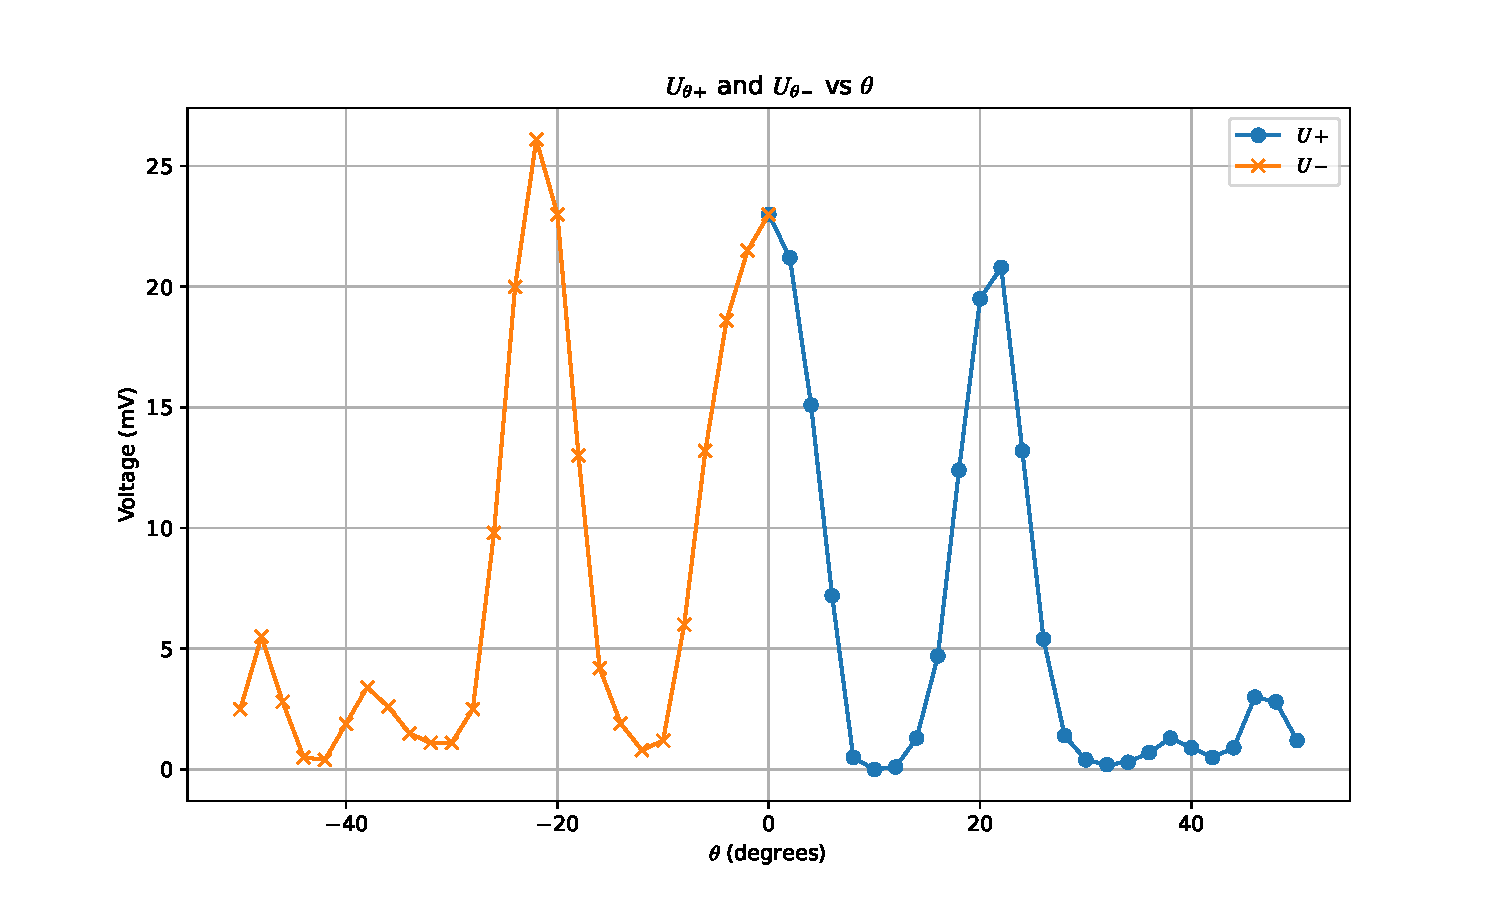
\includegraphics[width=0.8\textwidth]{双缝干涉-粗扫数据.pdf}
    \caption{双缝干涉-粗扫数据}
\end{figure}

由该图可以知道双缝干涉各个极大和极小的角度值, 分别在这些角度值附近进行细扫, 得到的数据如表3-表5所示, 根据这些数据, 我们可以绘制出双缝干涉强度与角度的关系曲线, 即图2-图4

\begin{table}[H]
\centering
\begin{tabular}{|c|c|c|c|c|c|c|c|c|c|}
\hline
$U_{\theta+}$ (mV) & 13.1 & 16.6 & 20.2 & 21.8 & 20.9 & 16.6.1 & 12.6 & 8.9 & 4.6 \\
\hline
$\theta$ ($^\circ$) & 18 & 19.0 & 20 & 21.0 & 22.0 & 23.0 & 24 & 25 & 26.0 \\
\hline
$U_{\theta-}$ (mV) & 12 & 18.2 & 23 & 25.2 & 26.7 & 24.8 & 20 & 15 & 9.6 \\
\hline
\end{tabular}
\caption{双缝干涉-一级极大}
\end{table}

\begin{figure}[H]
    \centering
    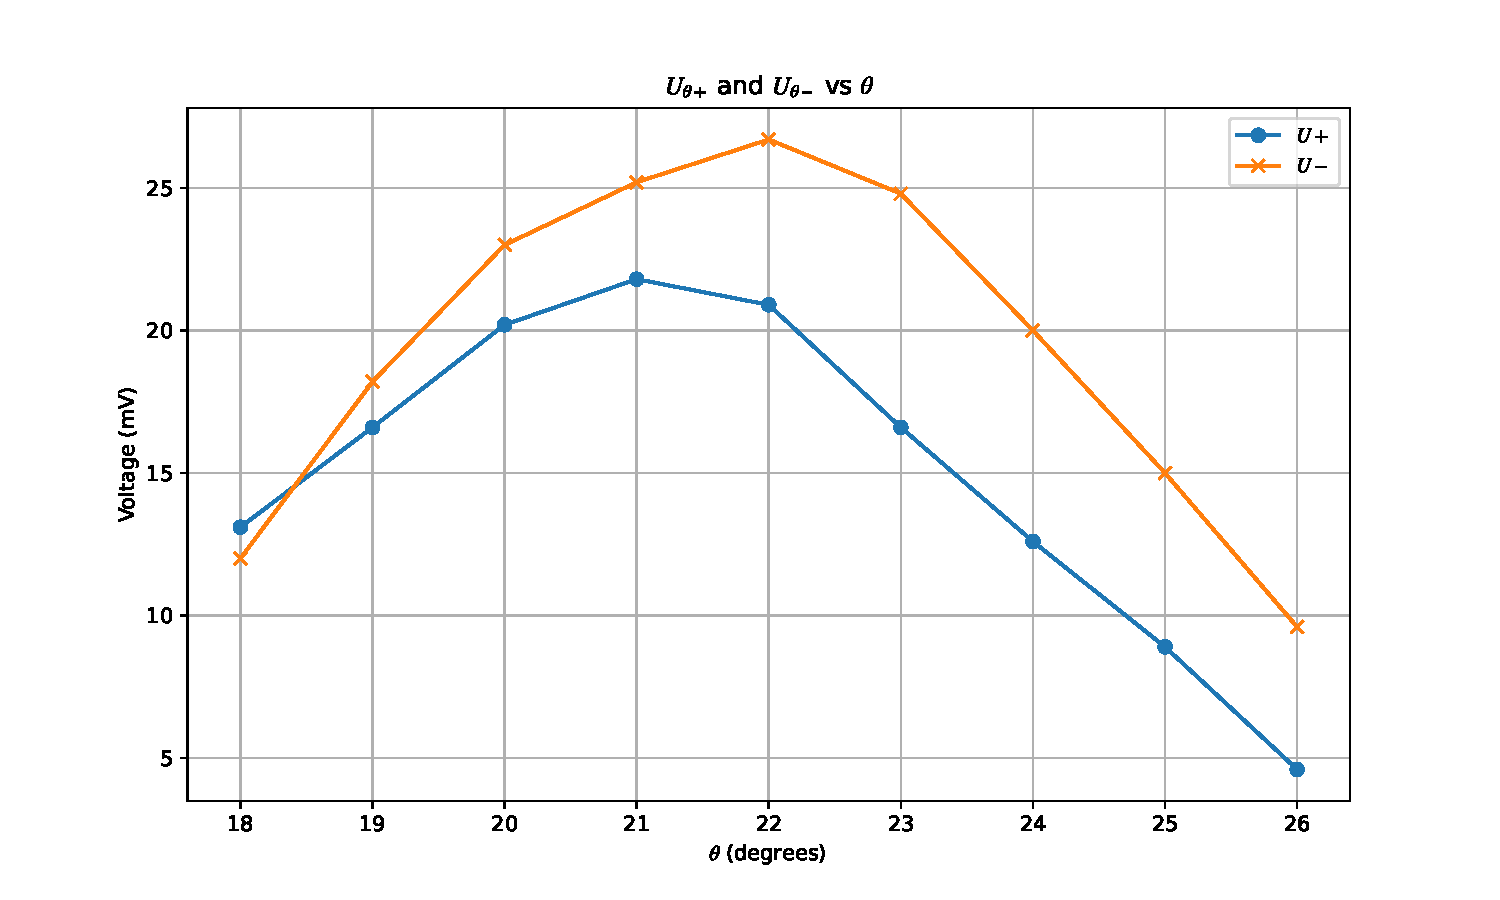
\includegraphics[width=0.75\textwidth]{双缝干涉-一级极大.pdf}
    \caption{双缝干涉-一级极大}
\end{figure}

取 $21^\circ$ 和 $22^\circ$ 为正一级极大和负一级极大的角度值, 取二者平均值 $21.5^\circ$ 作为一级极大的角度值, 根据公式（3.5）得到：

\[
\lambda = \frac{(\alpha + b) \sin \phi}{k} = \frac{(3.50 + 5.00) \times \sin 21.5^\circ}{1} = 3.1152 \, \text{cm}
\]

相对误差为：

\[
E_r = \frac{\lambda - \lambda_t}{\lambda_t} \times 100\% = \frac{(3.1152 - 3.1915)}{(3.1915)} \times 100\% = -2.39\%
\]

\begin{table}[H]
\centering
\begin{tabular}{|c|c|c|c|c|c|c|c|c|c|}
\hline
$U_{\theta+}$ (mV) & 2.3 & 0.5 & 0.1 & 0 & 0 & 0.2 & 0.6 & 1.1 & 2.5 \\
\hline
$\theta$ ($^\circ$) & 7 & 8.0 & 9.0 & 10.0 & 11.0 & 12.0 & 13.0 & 14.0 & 15 \\
\hline
$U_{\theta-}$ (mV) & 10 & 6.4 & 2.6 & 1.1 & 0.7 & 0.8 & 1.2 & 1.9 & 3 \\
\hline
\end{tabular}
\caption{双缝干涉-零级极小}
\end{table}


\begin{figure}[H]
    \centering
    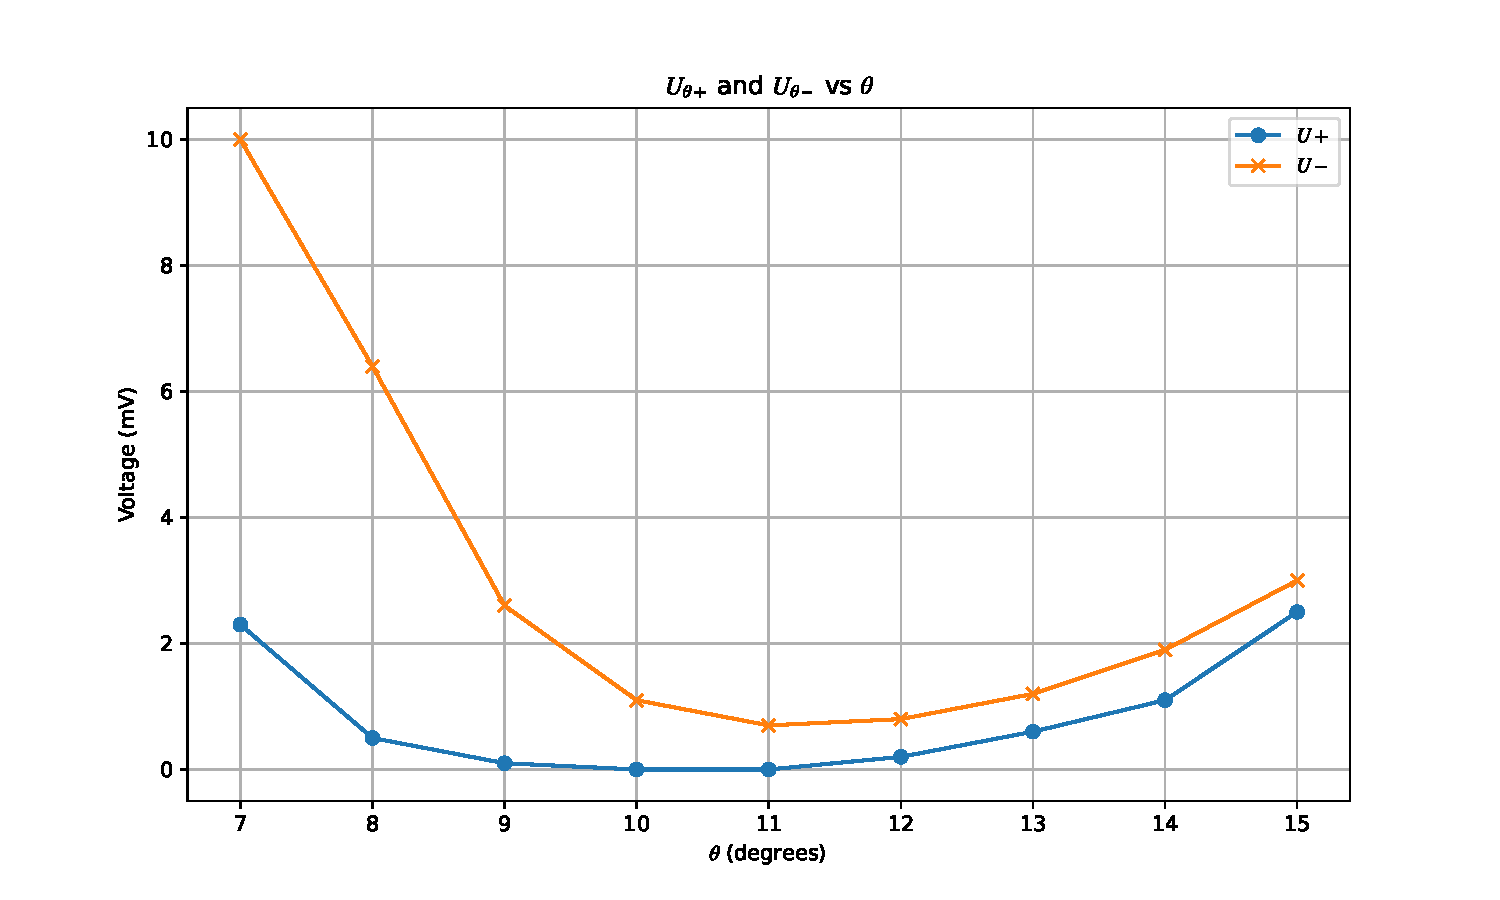
\includegraphics[width=0.75\textwidth]{双缝干涉-零级极小.pdf}
    \caption{双缝干涉-零级极小}
\end{figure}


取 $10.5^\circ$ 和 $11^\circ$ 为正零级极小和负零级极小的角度值, 取二者平均值 $10.75^\circ$ 作为一级极大的角度值, 根据公式（3.6）得到：

\[
\lambda = \frac{2(a + b) \sin \phi}{2k + 1} = \frac{2\times (3.50 + 5.00) \times \sin 10.75^\circ}{1} = 3.1709 \, \text{cm}
\]

相对误差为：

\[
E_r = \frac{\lambda - \lambda_t}{\lambda_t} \times 100\% = \frac{(3.1709 - 3.1915)}{(3.1915)} \times 100\% = -0.65\%
\]

\begin{table}[H]
\centering
\begin{tabular}{|c|c|c|c|c|c|c|c|c|c|}
\hline
$\theta$ ($^\circ$) & 28.0 & 29.0 & 30.0 & 31.0 & 32.0 & 33.0 & 34.0 & 35.0 & 36.0 \\
\hline
$U_{\theta+}$ (mV) & 1.3 & 0.6 & 0.4 & 0.3 & 0.2 & 0.2 & 0.3 & 0.5 & 0.8 \\
\hline
$\theta$ ($^\circ$) & 27.0 & 28.0 & 29.0 & 30.0 & 31.0 & 32.0 & 33.0 & 34.0 & 35.0 \\
\hline
$U_{\theta-}$ (mV) & 5.2 & 2.4 & 1.4 & 1.1 & 1.0 & 1.1 & 1.2 & 1.5 & 1.9 \\
\hline
\end{tabular}
\caption{双缝干涉-一级极小}
\end{table}



\begin{figure}[H]
    \centering
    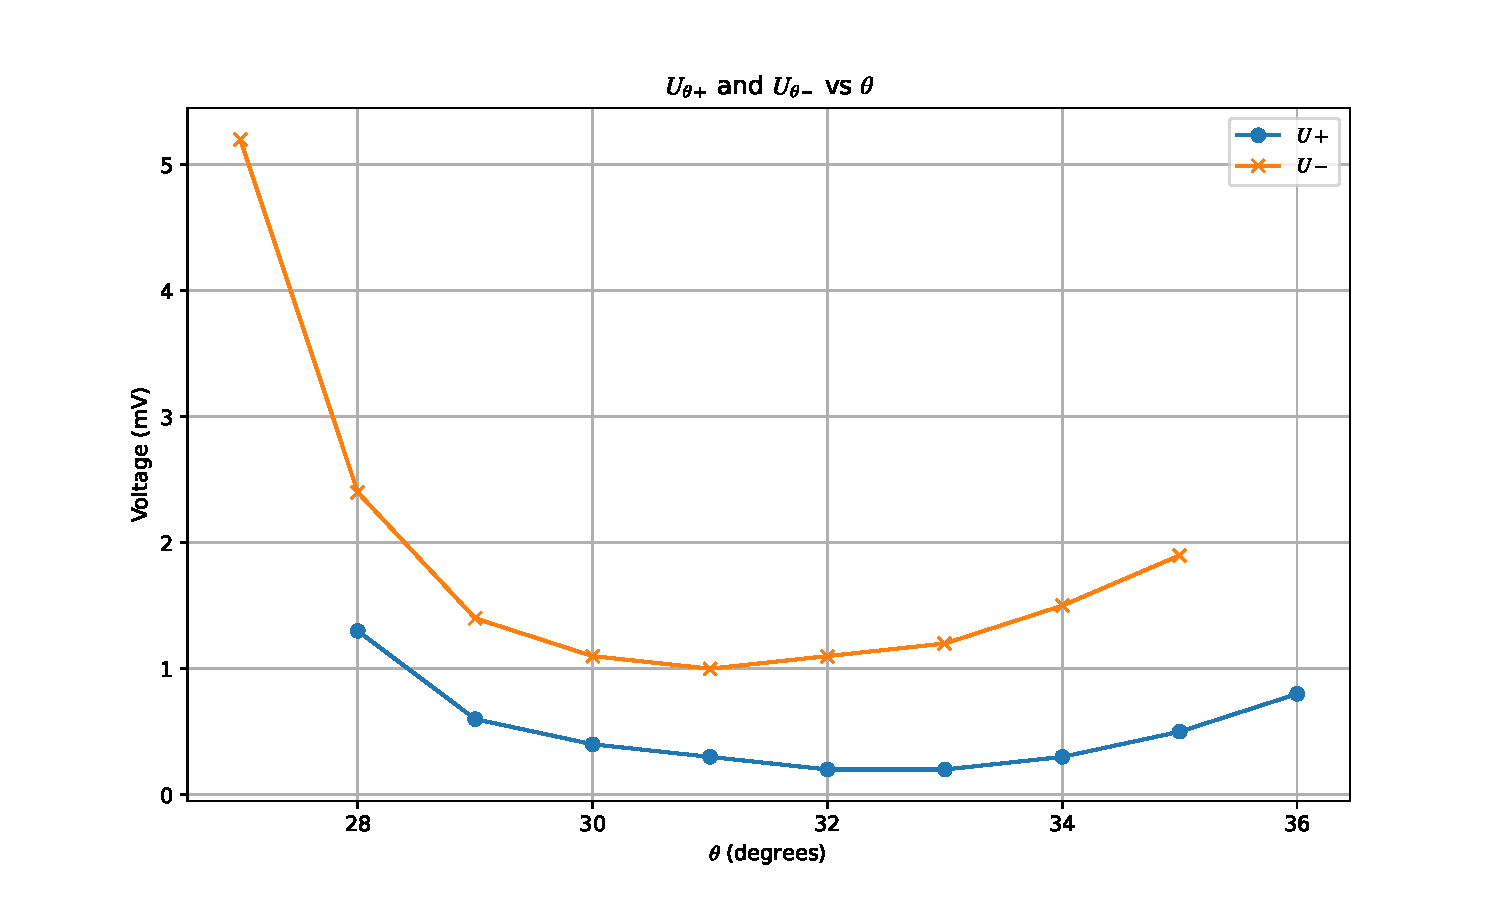
\includegraphics[width=0.8\textwidth]{双缝干涉-一级极小.pdf}
    \caption{双缝干涉-一级极小}
\end{figure}

取 $32^\circ$ 和 $31^\circ$ 为正零级极小和负零级极小的角度值, 取二者平均值 $31.5^\circ$ 作为一级极大的角度值, 根据公式（3.6）得到：

\[
\lambda = \frac{2(a + b) \sin \phi}{2k + 1} = \frac{2\times (3.50 + 5.00) \times \sin 31.5^\circ}{ 2 \times  1 + 1} = 2.9608 \, \text{cm}
\]

相对误差为：

\[
E_r = \frac{\lambda - \lambda_t}{\lambda_t} \times 100\% = \frac{(2.9608 - 3.1915)}{(3.1915)} \times 100\% = -7.23\%
\]
\subsection{微波的迈克尔逊干涉实验}
实验中读出当接收器接收的信号值最弱时反射板的位置如表6所示
\begin{table}[H]
\centering
\begin{tabular}{|c|c|c|c|c|}
\hline
最小读点数 (cm)  & 0.49 & 2.05 & 3.61 & 5.15 \\
\hline
\end{tabular}
\caption{迈克尔逊干涉原始数据}
\end{table}
对相邻两个最小读点数求差, 得到反射板每次移动的距离$\Delta x$, 并由此计算出微波波长 $\lambda = 2\Delta x$, 列得表7
\begin{table}[H]
\centering
\begin{tabular}{|c|c|c|c|}
\hline
移动距离$\Delta x$ (cm)  & 1.56 & 1.56 & 1.54 \\
\hline
波长$\lambda$ (cm)  & 3.12 & 3.12 & 3.08 \\
\hline
\end{tabular}
\caption{迈克尔逊干涉数据处理}
\end{table}

因此波长的平均值为
\[
\bar{\lambda} = \frac{1}{3} (3.12 + 3.12 + 3.08) = 3.11 \, \text{cm}.
\]

从而相对误差为
\[
E_r = \frac{\bar{\lambda} - \lambda_t}{\lambda_t} \times 100\% = \frac{3.11 - 3.1915}{3.1915} \times 100\% = 2.55\%.
\]
\subsection{微波布拉格衍射实验}
微波布拉格衍射实验的原始数据如表8-表11所示, 根据这些数据, 我们可以绘制出布拉格衍射强度与角度的关系曲线, 即图5-图8
\begin{table}[H]
\centering
\begin{tabular}{|c|c|c|c|c|c|c|c|c|c|}
\hline
$\Phi$ ($^\circ$) & 30.0 & 32.0 & 34.0 & 36.0 & 38.0 & 40.0 & 42.0 & 44.0 & 46.0 \\
\hline
$U$ (mV) & 1.8 & 2.1 & 1.8 & 2.2 & 4.8 & 9.2 & 5.7 & 1.2 & 0.8 \\
\hline
$\Phi$ ($^\circ$) & 48.0 & 50.0 & 52.0 & 54.0 & 56.0 & 58.0 & 60.0 & 62.0 & 64.0 \\
\hline
$U$ (mV) & 5.0 & 6.3 & 1.2 & 0.8 & 2.0 & 1.1 & 13.0 & 26.3 & 9.0 \\
\hline
$\Phi$ ($^\circ$) & 66.0 & 68.0 & 70.0 & 72.0 & 74.0 & 76.0 & 78.0 & 80.0 &   \\
\hline
$U$ (mV) & 57.2 & 97.2 & 30.7 & 1.1 & 2.6 & 15.2 & 0.2 & 11.0 &   \\
\hline
\end{tabular}
\caption{布拉格衍射-(100)面-粗扫数据}
\end{table}

\begin{figure}[H]
    \centering
    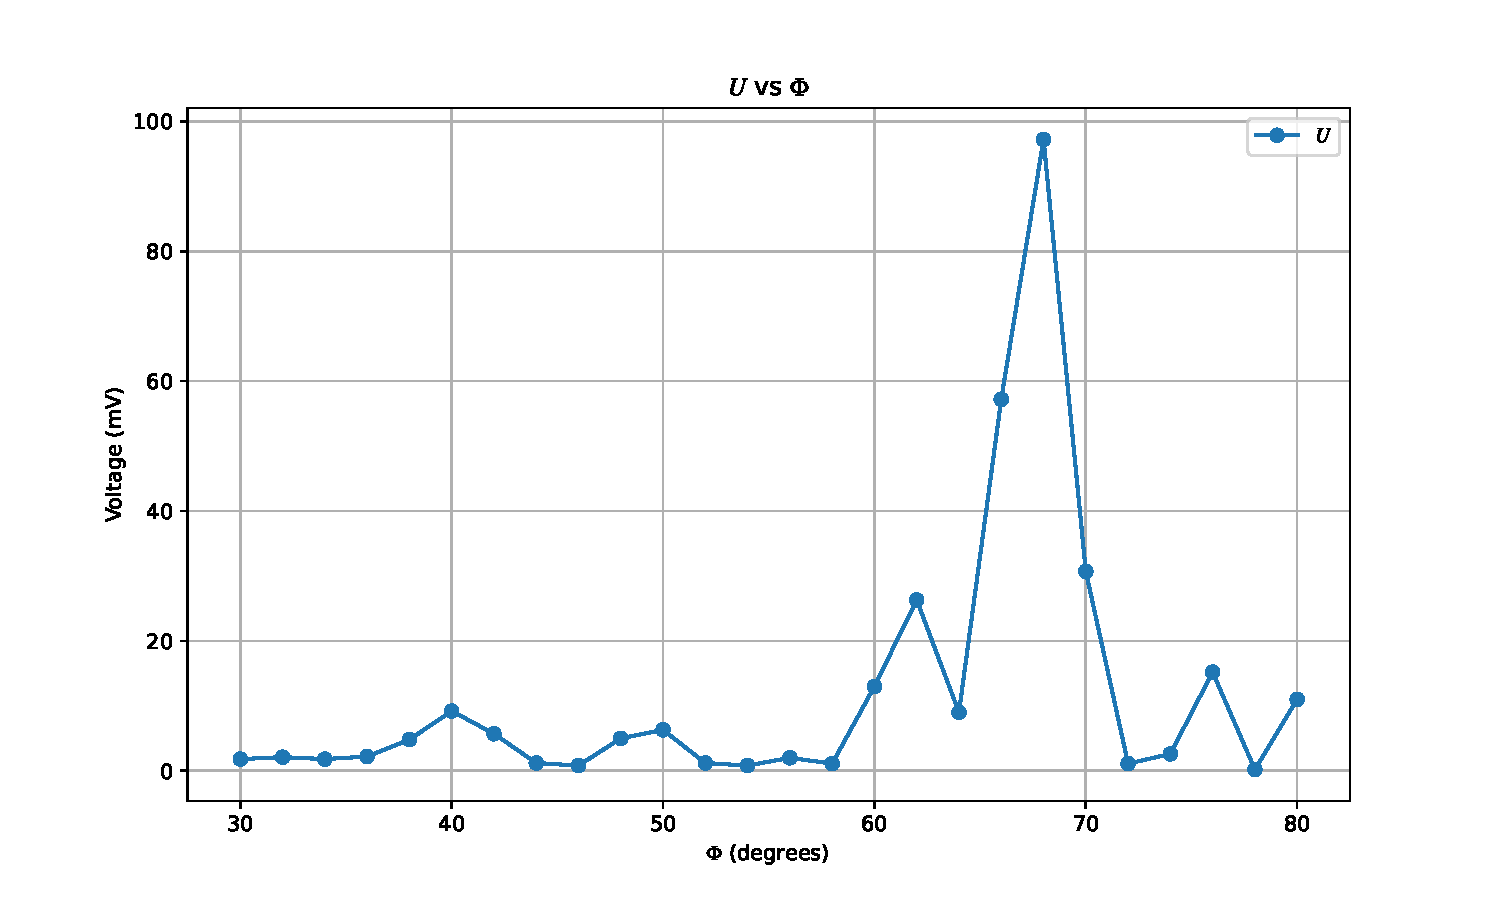
\includegraphics[width=0.75\textwidth]{布拉格衍射-(100)面-粗扫数据.pdf}
    \caption{布拉格衍射-(100)面-粗扫数据}
\end{figure}
根据图5, 我们可以知道布拉格衍射-(100)面各个极大和极小的角度值, 分别在这些角度值附近进行细扫, 可得到如下数据
\begin{table}[H]
\centering
\begin{tabular}{|c|c|c|c|c|c|c|c|c|c|}
\hline
$\Phi$ ($^\circ$) & 64.0 & 65.0 & 66.0 & 67 & 68.0 & 69.0 & 70.0 & 71.0 & 72 \\
\hline
$U$ (mV) & 9.9 & 28.2 & 59.4 & 81 & 98.1 & 83.9 & 30.6 & 2.6 & 1.0 \\
\hline
\end{tabular}
\caption{布拉格衍射-(100)面-极大}
\end{table}

\begin{figure}[H]
    \centering
    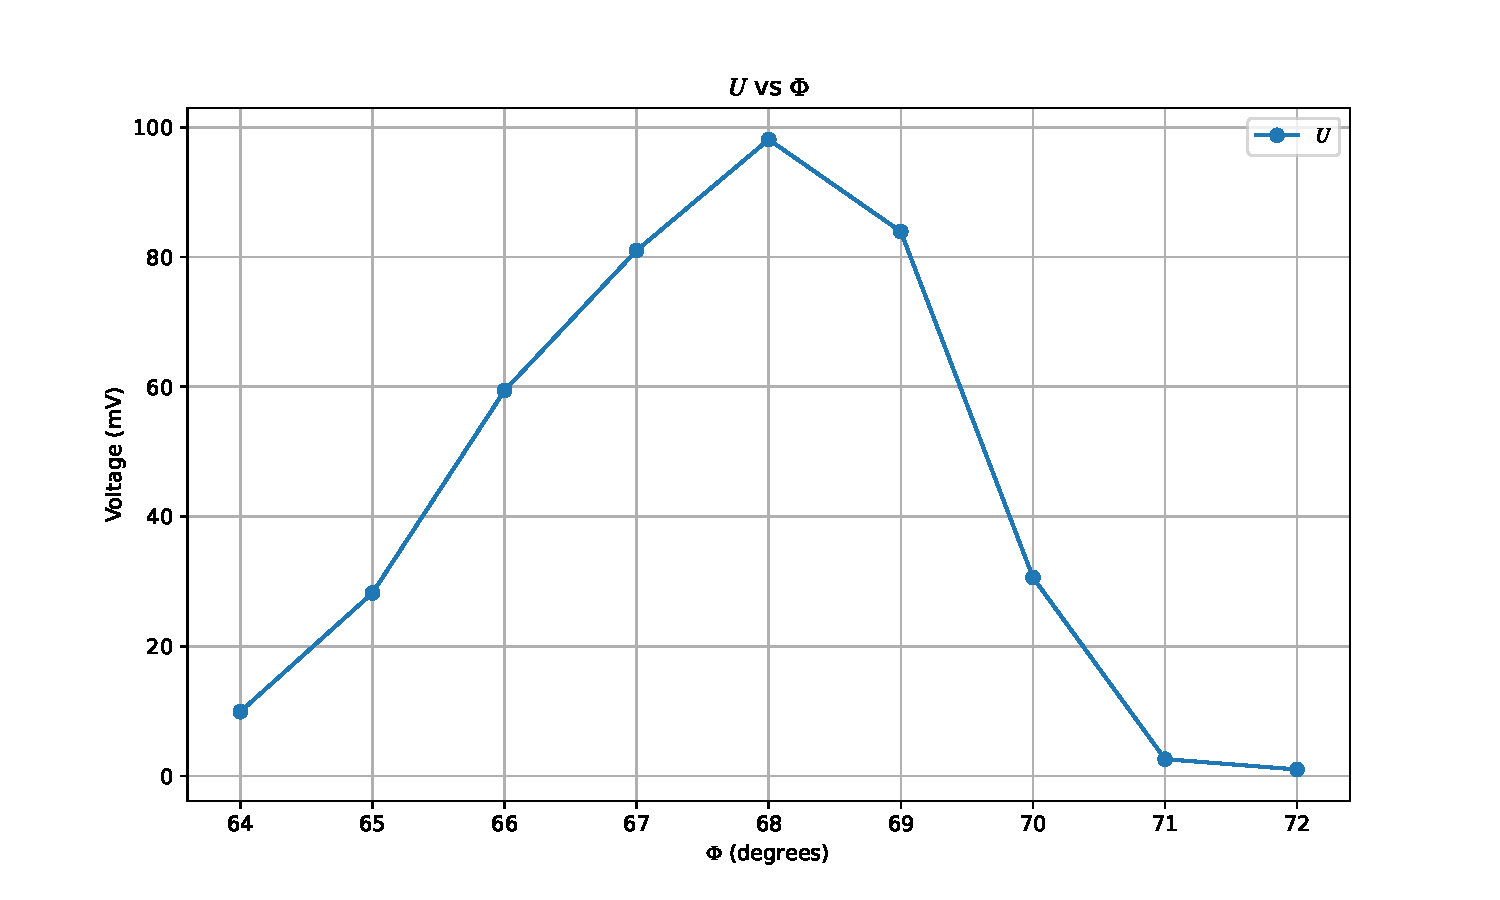
\includegraphics[width=0.75\textwidth]{布拉格衍射-(100)面-极大.pdf}
    \caption{布拉格衍射-(100)面-极大}
\end{figure}


可以看出极大值角度为 $68^\circ$. 利用根据公式 (3.2) 计算可以得到
\[
\lambda = \frac{2d \cos \beta}{k} = \frac{2 \times 4 \times \cos 68^\circ}{1} = 2.9969 \, \text{cm}.
\]
相对误差为
\[
E_r = \frac{\lambda - \lambda_t}{\lambda_t} \times 100\% = \frac{2.9969 - 3.1915}{3.1915} \times 100\% = -6.10\%.
\]

\begin{table}[H]
\centering
\begin{tabular}{|c|c|c|c|c|c|c|c|c|c|}
\hline
$\Phi$ ($^\circ$) & 30.0 & 32.0 & 34 & 36.0 & 38.0 & 40.0 & 42.0 & 44.0 & 46.0 \\
\hline
$U$ (mV) & 0.0 & 0.0 & 0 & 0.0 & 0.0 & 0.1 & 0.0 & 0.1 & 0.3 \\
\hline
$\Phi$ ($^\circ$) & 48.0 & 50.0 & 52 & 54.0 & 56.0 & 58.0 & 60.0 & 62.0 & 64.0 \\
\hline
$U$ (mV) & 0.2 & 0.5 & 2 & 4.7 & 4.7 & 4.0 & 2.6 & 0.1 & 0.3 \\
\hline
$\Phi$ ($^\circ$) & 66.0 & 68.0 & 70 &   &   &   &   &   &   \\
\hline
$U$ (mV) & 0.0 & 0.0 & 0.0 &   &   &   &   &   &   \\
\hline
\end{tabular}
\caption{布拉格衍射-(110)面-粗扫数据}
\end{table}


\begin{figure}[H]
    \centering
    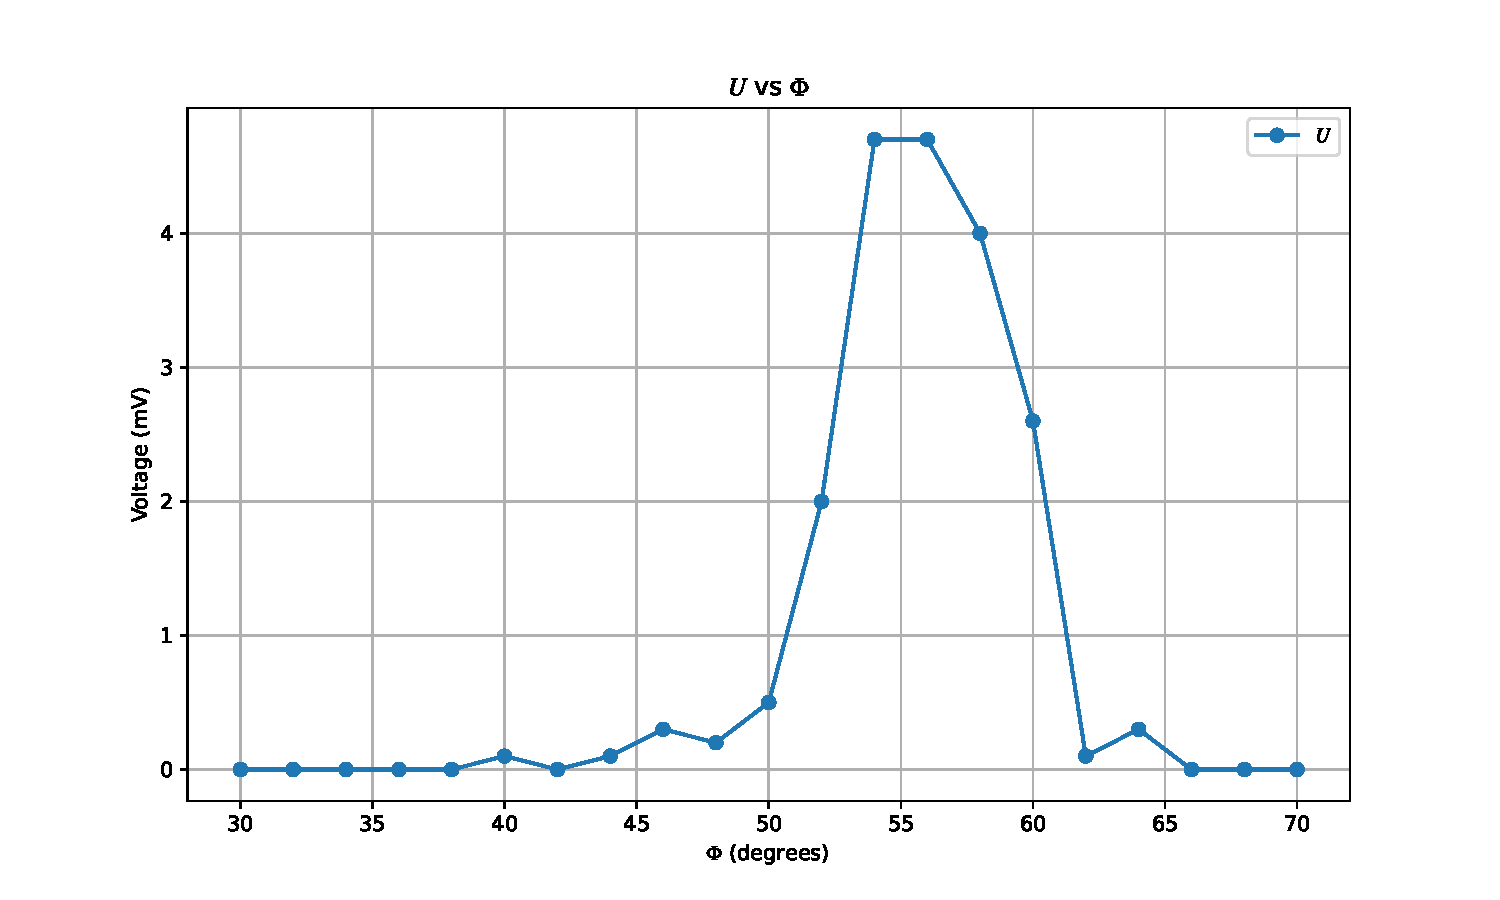
\includegraphics[width=0.75\textwidth]{布拉格衍射-(110)面-粗扫数据.pdf}
    \caption{布拉格衍射-(110)面-粗扫数据}
\end{figure}

根据图7, 我们可以知道布拉格衍射-(110)面各个极大和极小的角度值, 分别在这些角度值附近进行细扫, 可得到如下数据
\begin{table}[H]
\centering
\begin{tabular}{|c|c|c|c|c|c|c|c|c|c|}
\hline
$\Phi$ ($^\circ$) & 51.0 & 52.0 & 53.0 & 54.0 & 55.0 & 56.0 & 57.0 & 58 & 59.0 \\
\hline
$U$ (mV) & 1.3 & 1.9 & 2.9 & 4.7 & 6.1 & 4.7 & 4.2 & 4 & 3.1 \\
\hline
\end{tabular}
\caption{布拉格衍射-(110)面-极大}
\end{table}

\begin{figure}[H]
    \centering
    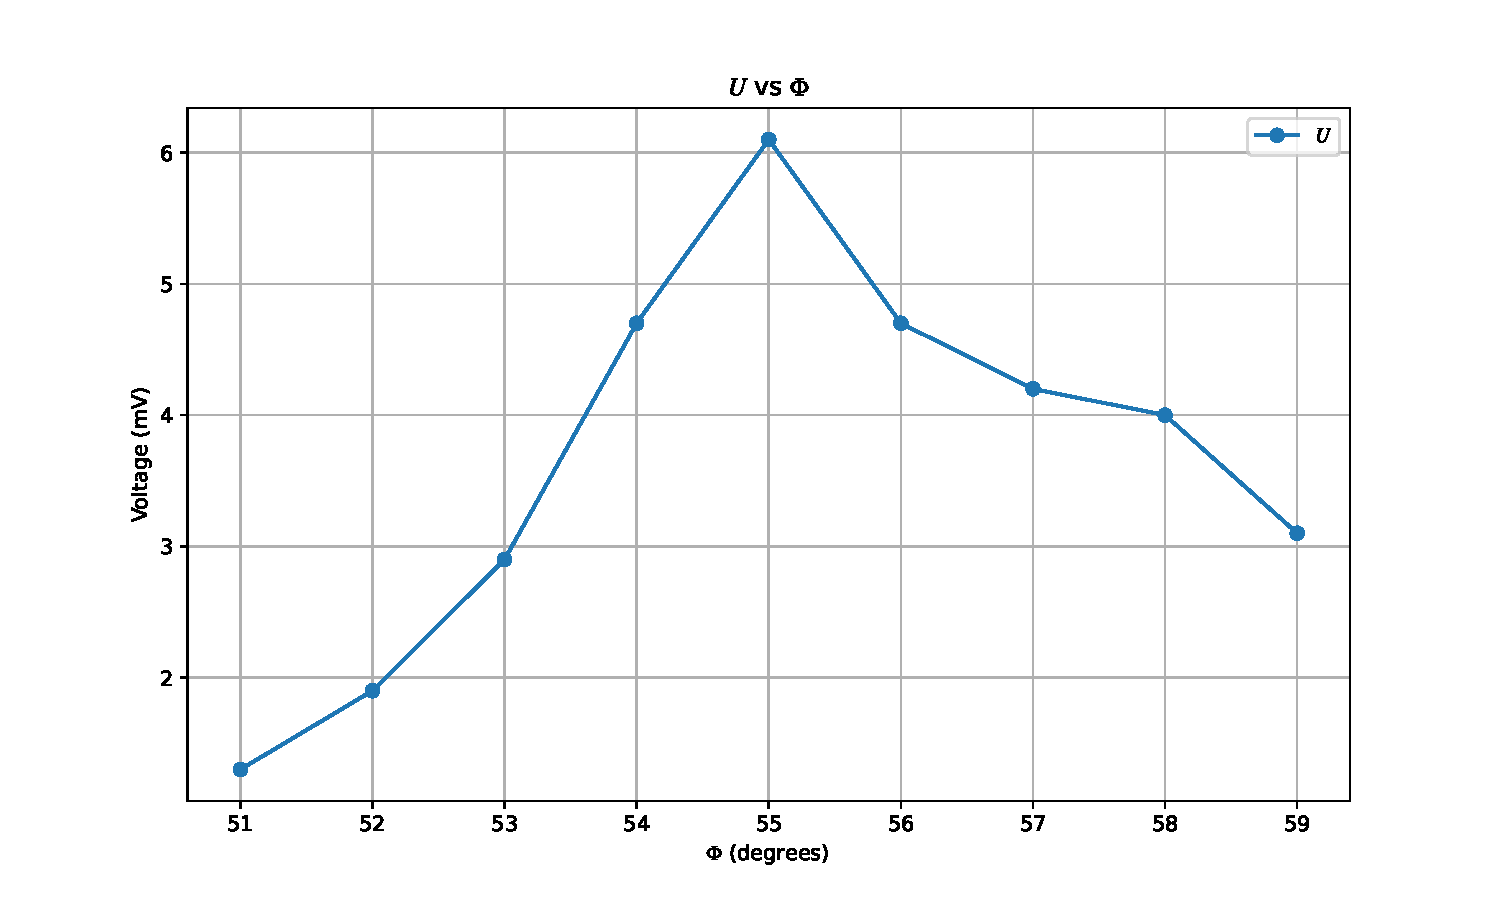
\includegraphics[width=0.75\textwidth]{布拉格衍射-(110)面-极大.pdf}
    \caption{布拉格衍射-(110)面-极大}
\end{figure}

可以看出极大值角度为 $55^\circ$. 利用根据公式 (3.2) 计算可以得到
\[
\lambda = \frac{2d \cos \beta}{k} = \frac{2 \times 2.828 \times \cos 55^\circ}{1} = 3.2441 \, \text{cm}.
\]
相对误差为
\[
E_r = \frac{\lambda - \lambda_t}{\lambda_t} \times 100\% = \frac{3.2441 - 3.1915}{3.1915} \times 100\% = 1.65\%.
\]
\section{实验总结和反思}
\subsection{实验总结}
在本次实验中, 我们使用了DHMS-1型微波光学综合实验仪进行测试. 实验主要通过安装和拆卸仪器、移动接收喇叭, 以及观察接收喇叭显示的电压值来进行. 为了减少误差, 实验过程中需要频繁校正接收喇叭的位置, 并且在移动接收喇叭时需缓慢进行, 以避免因移动而引起的位置偏移. 由于实验中需要记录大量数据, 因此良好的记录习惯显得尤为重要. 尽管在观测期间接收喇叭的数值会受到周围环境的影响而产生波动, 但只需在波动范围较小的情况下选择一个代表值即可, 无需长时间等待, 以免延长实验周期. 

在\textit{双缝干涉实验}中, 我们收集了大量数据, 努力确定一级极大、零级极小及一级极小对应的角度值. 初步获得角度值范围后, 我们进行了精细的范围缩小, 以提高实验的精度和准确性. 最终测量得到的数据误差范围相对较小, 但是我也注意到通过高级极大极小计算出来的波长误差远比低级极大极小计算出来的误差大, 我猜测这是因为测量高级极大极小时读到的电压值本身就相对较少, 仪器精度不够, 而更容易产生误差

在\textit{微波迈克尔逊干涉}实验中, 需要对多个仪器进行精确固定. 在测量过程中, 可能会出现多个连读度数都为$0$, 给最终选择实际的最小度数点带来了困难. 我发现可以通过加大发射源功率, 或者给多个零度数点取平均值来解决这个问题

在\textit{微波布拉格衍射实验}中, 会发现测量(110)面时相对于(100)面的测量数据普遍较小, 有效数据不是很多, 这可能是因为实验所用的模拟晶体在左右两侧有玻璃屏障, 使得部分微波被反射、吸收. 索性的的是尽管测量结果普遍较小, 但是最后计算出的波长的百分误差并不大.

\subsection{实验反思}
实验中的接收头难以被有效固定, 所以在移动接受头的臂的时候很容易不小心碰歪接收头, 导致一开始的对准失效, 需要重新对准进行实验. 因此在移动接受臂的时候必须要小心, 移动速度要慢, 尽量不要让手臂或者周围的吸音海绵发生碰撞

在测量数据时, 第二次的细扫中测量的数据有一般是和粗扫中一致或者是非常接近的, 所以如果能提升接受头的精度, 在细扫中采用更细的角度分割可能会产生更好的实验结果

\section{思考题}
\subsection{各实验内容误差主要影响是什么?}
实验中出现的误差主要源于以下几个方面：
\begin{enumerate}
    \item \textbf{接收喇叭位置偏移}：由于实验过程中频繁移动接收喇叭, 其位置可能发生微小偏移, 这会随着实验时间的推移而累积, 最终导致较大的误差. 尽管在实验准备时已将接收喇叭对齐, 但后续测量中左右数据常常出现不对称的情况. 
    
    \item \textbf{角度调节的误差}：实验中通过仪器的轮盘调整角度, 然而在调节过程中, 轮盘的无意触碰会造成位置的变化, 使得发射喇叭的角度难以与180°精确对齐. 同时, 由于肉眼观察的误差, 接收喇叭在需要的角度附近也可能发生偏移. 
    
    \item \textbf{双缝干涉实验中的误差}：双缝的安装位置无法完全与两个喇叭垂直, 这可能导致最终结果的不对称. 此外, 轮盘的微小偏移也对双缝的位置产生影响. 
    
    \item \textbf{微波迈克尔逊干涉实验中的误差}：由于安装位置不完全合适, 反射镜的手动移动会导致数据的变化与实际位置不同步, 观测到最小数据时手轮可能已超出理想位置, 从而影响测量精度. 
    
    \item \textbf{微波布拉格衍射实验}：模拟晶体的体积会遮挡部分刻度, 并且接收与发射喇叭的不对称角度可能导致计算失误, 进一步增加误差. 
\end{enumerate}
\subsection{金属是一种良好的微波反射器. 其它物质的反射特性如何? 是否有部分能量透过这些物质还是被吸收了? 比较导体与非导体的反射特性.  }
金属是一种非常有效的微波反射材料. 相较于金属, 像玻璃这样的其他材料具有较低的反射率和较高的透射率, 使得大部分能量能穿透这些材料, 仅有少量能量被吸收. 而水主要以吸收能量为主, 其反射率较高但透射率较低. 由于导体具备良好的导电性能, 相对介电常数相对较小, 按照关系式 $ n = \sqrt{\epsilon_r \mu_r} $ 可知, 导体对微波的折射率极小, 因此反射效果相当优秀. 相比之下, 非导体的反射性能较为逊色. 

\begin{table}[H]
    \centering
    \begin{tabular}{@{}lll@{}}
        \toprule
        材料   & 反射能力 \\ \midrule
        玻璃   & 低      \\
        金属   & 高      \\
        水     & 高      \\
        导体   & 高      \\
        非导体 & 低      \\ \bottomrule
    \end{tabular}
    \caption{不同材料的反射能力比较}
    \label{tab:reflectivity}
\end{table}

\subsection{避免每台仪器微波间的干扰, 使用吸波材料对每套设备进行了微波屏蔽, 请问吸波材料的工作机理是什么?与屏蔽微波波长的关系是什么?}
为了避免不同设备之间的微波干扰, 我们选用了泡沫角锥微波吸收材料. 根据近似关系 $ L/\lambda \approx 1 $, 吸波材料的锥体长度与屏蔽的微波波长相当, 从而使得微波辐射能够有效地进入材料内部而不被反射. 锥形的结构设计使得入射的微波在表面多次反射和折射, 最终抵达锥底, 摊叠的能量被充分吸收并转化为热能, 从而实现对微波的有效屏蔽. 

\begin{figure}[H]
    \centering
    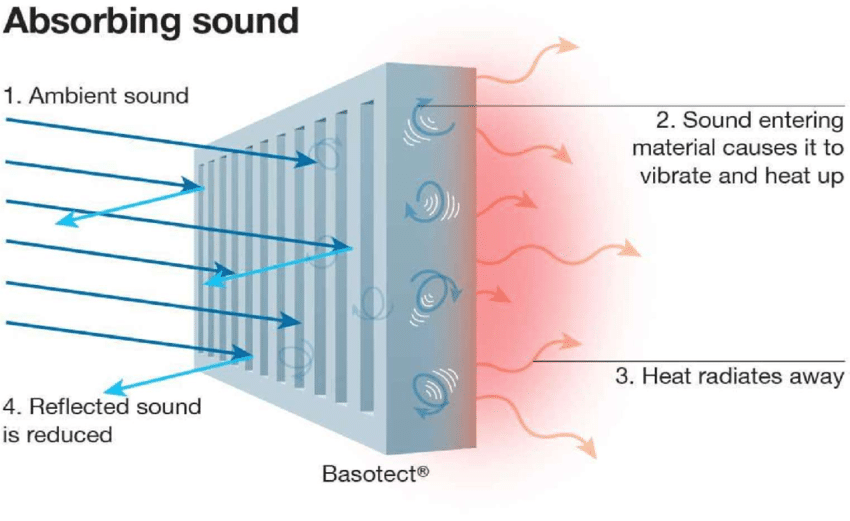
\includegraphics[width=0.8\textwidth]{Working-Principle-of-Acoustic-panel.png}
    \caption{吸波材料的工作机理}
\end{figure}

\subsection{假如预先不知道晶体中晶面的方向, 是否会增加实验的复杂性? 又该如何定位这些晶面? }
晶面方向的不确定性确实增加了实验操作的复杂程度. 当晶面的方向未知时, 自由度将扩展为三个, 增加了研究的复杂性. 确立晶面的位置的方法包括观察单晶切片或通过多次实验对比晶体在不同方向上的反射特性. 
\end{document}
